%%%%%%%%%%%%%%%%%%%%%%%%%%%%%%%%%%%%%%%%%
% Formal Book Title Page
% LaTeX Template
% Version 2.0 (23/7/17)
%
% This template was downloaded from:
% http://www.LaTeXTemplates.com
%
% Original author:
% Peter Wilson (herries.press@earthlink.net) with modifications by:
% Vel (vel@latextemplates.com)
%
% License:
% CC BY-NC-SA 3.0 (http://creativecommons.org/licenses/by-nc-sa/3.0/)
% 
% This template can be used in one of two ways:
%
% 1) Content can be added at the end of this file just before the \end{document}
% to use this title page as the starting point for your document.
%
% 2) Alternatively, if you already have a document which you wish to add this
% title page to, copy everything between the \begin{document} and
% \end{document} and paste it where you would like the title page in your
% document. You will then need to insert the packages and document 
% configurations into your document carefully making sure you are not loading
% the same package twice and that there are no clashes.
%
%%%%%%%%%%%%%%%%%%%%%%%%%%%%%%%%%%%%%%%%%

%----------------------------------------------------------------------------------------
%	PACKAGES AND OTHER DOCUMENT CONFIGURATIONS
%----------------------------------------------------------------------------------------

\documentclass[a4paper, 11pt, oneside]{article} % A4 paper size, default 11pt font size and oneside for equal margins

\newcommand{\plogo}{\fbox{$\mathcal{PL}$}} % Generic dummy publisher logo

\usepackage{CJKutf8}
\usepackage[utf8]{inputenc} % Required for inputting international characters
\usepackage[T1]{fontenc} % Output font encoding for international characters
\usepackage{fouriernc} % Use the New Century Schoolbook font
\usepackage{amsmath}
\usepackage{graphicx}
\usepackage{subcaption}
\usepackage{enumitem}
\usepackage{multicol}
\usepackage{tikz}
\usepackage{mathtools}
\usepackage{hyperref}
\usepackage{listings}


%----------------------------------------------------------------------------------------
%	TITLE PAGE
%----------------------------------------------------------------------------------------

\begin{document} 

\begin{titlepage} % Suppresses headers and footers on the title page

	\centering % Centre everything on the title page
	
	\scshape % Use small caps for all text on the title page
	
	\vspace*{\baselineskip} % White space at the top of the page

	\begin{figure}

        \centering

        
\includegraphics[width=0.7\textwidth]{../output/logo}

    \end{figure}
	
	%------------------------------------------------
	%	Title
	%------------------------------------------------
	
	\rule{\textwidth}{1.6pt}\vspace*{-\baselineskip}\vspace*{2pt} % Thick horizontal rule
	\rule{\textwidth}{0.4pt} % Thin horizontal rule
	
	\vspace{0.75\baselineskip} % Whitespace above the title
	
	{\LARGE Human Information Data Mining} % Title
	
	\vspace{0.75\baselineskip} % Whitespace below the title
	
	\rule{\textwidth}{0.4pt}\vspace*{-\baselineskip}\vspace{3.2pt} % Thin horizontal rule
	\rule{\textwidth}{1.6pt} % Thick horizontal rule
	
	\vspace{2\baselineskip} % Whitespace after the title block
	
	%------------------------------------------------
	%	Subtitle
	%------------------------------------------------
	
	Homework 2 % Subtitle or further description
	
	\vspace*{3\baselineskip} % Whitespace under the subtitle
	
	%------------------------------------------------
	%	Editor(s)
	%------------------------------------------------
	
	Student ID:

	\vspace{0.5\baselineskip}

	{\scshape 108368017}

	\vspace{0.5\baselineskip}

	Student: 
	
	\vspace{0.5\baselineskip} % Whitespace before the editors

	% {\scshape 108368017 \hspace{10mm}}
	{\scshape\Large Zi-Yang Lin } % Editor list

	\vspace{0.5\baselineskip} % Whitespace before the editors


	Advisor:

	\vspace{0.5\baselineskip} % Whitespace before the editors
	
	{\scshape\Large Jenq-Haur Wang} % Editor list
	
	\vspace{0.5\baselineskip} % Whitespace below the editor list
	
	\textit{National Taipei University of Technology} % Editor affiliation
	
	\vfill % Whitespace between editor names and publisher logo
	
	%------------------------------------------------
	%	Publisher
	%------------------------------------------------
	
	% \plogo % Publisher logo
	
	\vspace{0.3\baselineskip} % Whitespace under the publisher logo
	
	2019 % Publication year
	
	% {\large publisher} % Publisher

\end{titlepage}

%----------------------------------------------------------------------------------------

\clearpage

\section*{Problem 1}
\textbf{6.6:} A database has five transactions. Let $min\_sup=60\% \quad and \quad min\_conf=80\%$.

\begin{center}
\begin{tabular}{ |c|c| } 
	\hline
	TID & Items bought \\
	\hline
		T100 & M, O, N, K, E, Y \\
		T200 & D, O, N, K, E, Y \\
		T300 & M, A, K, E \\
		T400 & M, U, C, K, Y \\
		T500 & C, O, O, K, I, E \\
	\hline
\end{tabular}
\end{center}

\begin{enumerate}[label=(\alph*)]

	\item Find all frequent itemsets using Apriori and FP-growth, respectively.
	Compare the efficiency of the two mining processes.
	\subsection*{Ans:}
	Apriori Algorithm:
	\begin{figure}[h!]
		\centering
		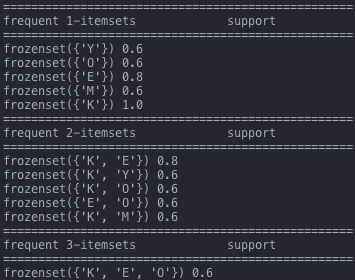
\includegraphics[width=\textwidth]{../output/apriori}
		\caption{Apriori algorithm result}
		\label{fig:empirical-distribution}
	\end{figure}

\clearpage

	FP-growth tree:

	\begin{center}
	\begin{tikzpicture}[level distance=1.8cm,
		level 1/.style={sibling distance=3.0cm},
		level 2/.style={sibling distance=5.0cm},
		level 3/.style={sibling distance=4.0cm},
		level 4/.style={sibling distance=1.2cm},
		level 5/.style={sibling distance=0.9cm}]
	\tikzstyle{every node}=[circle, draw]
		\node (Root) {root}
			child {
				node {$K:5$} 
				child { node (a1) {$E:4$}
					child { node {$M:2$}
						child { node {$O:1$}
							child { node {$Y:1$}}
						}
					}
					child { node {$O:2$}
						child { node {$Y:1$}}
					}
				}
				child { node (a2) {$M:1$}
					child { node {$Y:1$}}
				}
			};
	\end{tikzpicture}
	\end{center}

	Apriori has to do multiple scans of the database while FP-growth builds the FP-Tree with
	a single scan. Candidate generation in Apriori is expensive (owing to the self-join), 
	while FP-growth does not generate any candidates.

\clearpage

	\item List all the strong association rules (with support s and confidence c) matching the following metarule, 
	where X is a variable representing customers, and $item_i$ denotes variables representing items (e.g. “A”, “B”):
	
	\begin{align*}
		\forall X \in transaction, buys(X, item_1) \cap buys(X, item_2) \Rightarrow buys(X, item_3)		[s, c]
	\end{align*}

	\subsection*{Ans:}

	\begin{align*}
		buys(X, E) \quad and \quad buys(X, O) \Rightarrow buys(X, K) \quad [60\%, 100\%] \\
		buys(X, O) \quad and \quad buys(X, K) \Rightarrow buys(X, E) \quad [60\%, 100\%]
	\end{align*}	

\end{enumerate}

\clearpage

\section*{Problem 2}
\textbf{6.8:} A database has four transactions. Let $min\_sup=60\% \quad and \quad min\_conf=80\%$.

\begin{center}
	\begin{tabular}{ |c|c|l| } 
		\hline
		Cust ID & TID & Items bought (in the form of brand-item category) \\
		\hline
			01 & T100 & King’s-Crab, Sunset-Milk, Dairyland-Cheese, Best-Bread \\
			02 & T200 & Best-Cheese, Dairyland-Milk, Goldenfarm-Apple, \\
			   &      & Tasty-Pie, Wonder-Bread \\
			01 & T300 & Westcoast-Apple, Dairyland-Milk, Wonder-Bread, Tasty-Pie \\
			03 & T400 & Wonder-Bread, Sunset-Milk, Dairyland-Cheese \\
		\hline
	\end{tabular}
\end{center}

\begin{enumerate}[label=(\alph*)]

	\item At the granularity of item\_category, (e.g. $item_i$ could be ``Milk''), for the rule template,
	
	\begin{align*}
		\forall X \in transaction, buys(X, item_1) \cap buys(X, item_2) \Rightarrow buys(X, item_3)		[s, c]
	\end{align*}

	list the frequent k-itemset for the largest k, and all the strong association rules 
	(with their support s and confidence c) containing the frequent k-itemset for the largest k.
	
	\subsection*{Ans:}

	\begin{align*}
	\begin{gathered}
		k = 3 \\
		frequent \quad 3 - itemset \quad is \quad \{Bread, \quad Milk, \quad Cheese\} \\
		Bread \cap Cheese \quad \Rightarrow \quad Milk \quad [75\%, \quad 100\%] \\
		Cheese \cap Milk \quad \Rightarrow \quad Bread \quad [75\%, \quad 100\%] \\
		Cheese \quad \Rightarrow \quad Milk \cap Bread \quad [75\%, \quad 100\%] \\
	\end{gathered}
	\end{align*}

\clearpage

	\item At the granularity of brand-item\_category, (e.g. $item_i$ could be ``Sunset-Milk''), for the rule template, 
	
	\begin{align*}
		\forall X \in transaction, buys(X, item_1) \cap buys(X, item_2) \Rightarrow buys(X, item_3)		[s, c]
	\end{align*}

	list the frequent k-itemset for the largest k (but do not print any rules).

	\subsection*{Ans:}

	\begin{align*}
	\begin{gathered}
		k = 3 \\
		frequent \quad 3 - itemset \quad is \\ \{(Wonder-Bread, \quad Dairyland-Milk, 
		\quad Tasty-Pie) \\ (Wonder-Bread, \quad Sunset-Milk, \quad Dairyland-Cheese)\}
	\end{gathered}
	\end{align*}

\end{enumerate}

\clearpage

\section*{Problem 3}
\textbf{6.14:} The following contingency table summarizes supermarket transaction data, 
where hot dogs refers to the transactions containing hot dogs, 
!(hot dogs) refers to the transactions that do not contain hot dogs, 
hamburgers refers to the transactions containing hamburgers, 
!(hamburgers) refers to the transactions that do not contain hamburgers.

\begin{center}
	\begin{tabular}{ |c|c|c|c| } 
		\hline
		 & hot dogs & !(hot dogs) & total \\
		\hline
			hamburgers & 2000 & 500 & 2500 \\
			!(hamburgers) & 1000 & 1500 & 2500 \\
			Total & 3000 & 2000 & 5000 \\
		\hline
	\end{tabular}
\end{center}

\begin{enumerate}[label=(\alph*)]

	\item Suppose that the association rule ``hot dogs $\Rightarrow$ hamburgers'' is mined. 
	Given a minimum support threshold of 25\% and a minimum confidence threshold of 50\%, 
	is this association rule strong?

	\subsection*{Ans:}

	For the rule, $support = 2000/5000 = 40\%$, \\
	and $confidence = 2000/3000 = 66.7\%$. \\
	Therefore, the assocation rule is strong.

	\item Based on the given data, is the purchase of hot dogs independent of 
	the purchase of hamburgers? If not, 
	what kind of correlation relationship exists between the two?

	\subsection*{Ans:}

	\begin{align*}
	\begin{gathered}
		correlation_{(hot dog, hamburgers)} \\
		= P(\{hot dog, hamburger\}) / P(\{hot dog\}) P(\{hamburger\}) \\
		= 0.4 / (0.6 \times 0.5) = 1.33 > 1
	\end{gathered}
	\end{align*}

	So, the purchase of hot dogs is not independent of purchase of hamburgers.
	There exists a positive correlation between the two.

	\item Compare the use of cosine measures with lift and correlation on the given data.
	
	\subsection*{Ans:}

	\begin{align*}
	\begin{gathered}
		cosine = P(\{hot dog, hamburger\}) / \sqrt{P(\{hot dog\}) P(\{hamburger\})} \\
		= 0.4 / \sqrt{0.6 \times 0.5} = 0.7 \quad (Positively \quad Correlated)  \\
	\end{gathered}
	\end{align*}

\end{enumerate}

\end{document}
